% Template for PLoS
% Version 3.1 February 2015
%
% To compile to pdf, run:
% latex plos.template
% bibtex plos.template
% latex plos.template
% latex plos.template
% dvipdf plos.template
%
% % % % % % % % % % % % % % % % % % % % % %
%
% -- IMPORTANT NOTE
%
% This template contains comments intended 
% to minimize problems and delays during our production 
% process. Please follow the template instructions
% whenever possible.
%
% % % % % % % % % % % % % % % % % % % % % % % 
%
% Once your paper is accepted for publication, 
% PLEASE REMOVE ALL TRACKED CHANGES in this file and leave only
% the final text of your manuscript.
%
% There are no restrictions on package use within the LaTeX files except that 
% no packages listed in the template may be deleted.
%
% Please do not include colors or graphics in the text.
%
% Please do not create a heading level below \subsection. For 3rd level headings, use \paragraph{}.
%
% % % % % % % % % % % % % % % % % % % % % % %
%
% -- FIGURES AND TABLES
%
% Please include tables/figure captions directly after the paragraph where they are first cited in the text.
%
% DO NOT INCLUDE GRAPHICS IN YOUR MANUSCRIPT
% - Figures should be uploaded separately from your manuscript file. 
% - Figures generated using LaTeX should be extracted and removed from the PDF before submission. 
% - Figures containing multiple panels/subfigures must be combined into one image file before submission.
% For figure citations, please use "Fig." instead of "Figure".
% See http://www.plosone.org/static/figureGuidelines for PLOS figure guidelines.
%
% Tables should be cell-based and may not contain:
% - tabs/spacing/line breaks within cells to alter layout or alignment
% - vertically-merged cells (no tabular environments within tabular environments, do not use \multirow)
% - colors, shading, or graphic objects
% See http://www.plosone.org/static/figureGuidelines#tables for table guidelines.
%
% For tables that exceed the width of the text column, use the adjustwidth environment as illustrated in the example table in text below.
%
% % % % % % % % % % % % % % % % % % % % % % % %
%
% -- EQUATIONS, MATH SYMBOLS, SUBSCRIPTS, AND SUPERSCRIPTS
%
% IMPORTANT
% Below are a few tips to help format your equations and other special characters according to our specifications. For more tips to help reduce the possibility of formatting errors during conversion, please see our LaTeX guidelines at http://www.plosone.org/static/latexGuidelines
%
% Please be sure to include all portions of an equation in the math environment.
%
% Do not include text that is not math in the math environment. For example, CO2 will be CO\textsubscript{2}.
%
% Please add line breaks to long display equations when possible in order to fit size of the column. 
%
% For inline equations, please do not include punctuation (commas, etc) within the math environment unless this is part of the equation.
%
% % % % % % % % % % % % % % % % % % % % % % % % 
%
% Please contact latex@plos.org with any questions.
%
% % % % % % % % % % % % % % % % % % % % % % % %

\documentclass[10pt,letterpaper]{article}
\usepackage[top=0.85in,left=2.75in,footskip=0.75in]{geometry}

% Use adjustwidth environment to exceed column width (see example table in text)
\usepackage{changepage}

% Use Unicode characters when possible
\usepackage[utf8]{inputenc}

% textcomp package and marvosym package for additional characters
\usepackage{textcomp,marvosym}

% fixltx2e package for \textsubscript
\usepackage{fixltx2e}

% amsmath and amssymb packages, useful for mathematical formulas and symbols
\usepackage{amsmath,amssymb}

% cite package, to clean up citations in the main text. Do not remove.
\usepackage{cite}

% Use nameref to cite supporting information files (see Supporting Information section for more info)
\usepackage{nameref,hyperref}

% line numbers
\usepackage[right]{lineno}

% ligatures disabled
\usepackage{microtype}
\DisableLigatures[f]{encoding = *, family = * }

% rotating package for sideways tables
\usepackage{rotating}

% Remove comment for double spacing
%\usepackage{setspace} 
%\doublespacing

% Text layout
\raggedright
\setlength{\parindent}{0.5cm}
\textwidth 5.25in 
\textheight 8.75in

% Bold the 'Figure #' in the caption and separate it from the title/caption with a period
% Captions will be left justified
\usepackage[aboveskip=1pt,labelfont=bf,labelsep=period,justification=raggedright,singlelinecheck=off]{caption}

% Use the PLoS provided BiBTeX style
\bibliographystyle{plos2015}

%%%%%%%%%%%%%%%%%%%%%%% START - MY SETUP %%%%%%%%%%%%%%%%%%%%%%%%%%%%%%

\usepackage{url}\urlstyle{same}
\usepackage{booktabs}
\usepackage{colortbl, xcolor}
\usepackage{epstopdf}

% rysunki
\usepackage{tikz}
\usepackage{ifthen}
\usepackage{xxcolor}
\usetikzlibrary{arrows}
\usetikzlibrary[topaths]
\usetikzlibrary{decorations.pathreplacing}

%%%%%%%%%%%%%%%%%%%%%%% END - MY SETUP %%%%%%%%%%%%%%%%%%%%%%%%%%%%%%

% Remove brackets from numbering in List of References
\makeatletter
\renewcommand{\@biblabel}[1]{\quad#1.}
\makeatother

% Leave date blank
\date{}

% Header and Footer with logo
\usepackage{lastpage,fancyhdr,graphicx}
\usepackage{epstopdf}
\pagestyle{myheadings}
\pagestyle{fancy}
\fancyhf{}
\lhead{
\includegraphics[width=2.0in]{PLOS-submission.eps}}
\rfoot{\thepage/\pageref{LastPage}}
\renewcommand{\footrule}{\hrule height 2pt \vspace{2mm}}
\fancyheadoffset[L]{2.25in}
\fancyfootoffset[L]{2.25in}
\lfoot{\sf PLOS}

%% Include all macros below

\newcommand{\lorem}{{\bf LOREM}}
\newcommand{\ipsum}{{\bf IPSUM}}

%% END MACROS SECTION


\begin{document}
\vspace*{0.35in}

% Title must be 250 characters or less.
% Please capitalize all terms in the title except conjunctions, prepositions, and articles.
\begin{flushleft}
{\Large
\textbf\newline{Prediction of malarial signal peptides}
}
\newline
% Insert author names, affiliations and corresponding author email (do not include titles, positions, or degrees).
\\
Micha\l{}  Burdukiewicz\textsuperscript{1},
Piotr Sobczyk\textsuperscript{2},
Pawe\l{} B\l{}a\.{z}ej\textsuperscript{1},
Pawe\l{} Mackiewicz*\textsuperscript{1},
\\
\bigskip
\bf{1} University of Wroc\l{}aw, Department of Genomics, Poland
\\
\bf{2} Wroc\l{}aw University of Technology, Department of Mathematics, Poland
\\
\bigskip

% Use the asterisk to denote corresponding authorship and provide email address in note below.
* pamac@smorfland.uni.wroc.pl

\end{flushleft}
% Please keep the abstract below 300 words
\section*{Abstract}
Signal peptides play an essential role in targeting of proteins to endomembrane system and their export outside the cell. The proteins equipped with such peptides are of great importance in metabolism, maintenance of tissue structure, immune response and regulation of other organismal functions. These peptides may be recognized with adequate accuracy using learning systems. However, existing signal peptide predictors do not perform well on atypical signal peptides of the parasites belonging to the phylum Apicomplexa. That is why, we designed a new more universal probabilistic model for eukaryotic signal peptides, which includes knowledge about their organization, amino acid composition and variability. The proposed approach called signalHsmm is based on hidden semi-Markov models (HSMMs) and uses intrinsic knowledge about signal peptides. It is able to recognize signal peptides from malaria parasites \textit{Plasmodium} and their relatives more accurately (with AUC = 0.93) than popular programs (0.79). Moreover, our model showed the largest AUC = 0.97 on the eukaryotic sequences in comparison to other signal peptide predictor even when trained on very small data sets. Moreover, it proved to be very stable regardless of types of learning data. Therefore, our model does not need to be permanently retrained with the continuous expansion of sequence databases. The web-server of signalHsmm is available at \url{http://smorfland.uni.wroc.pl/signalhsmm}.


% Please keep the Author Summary between 150 and 200 words
% Use first person. PLOS ONE authors please skip this step. 
% Author Summary not valid for PLOS ONE submissions.   
\section*{Author Summary}


\linenumbers

\section*{Introduction}
\subsection*{Roles and features of signal peptides}

Proteins of eukaryotes are encoded in nuclear genomes and are synthesized in ribosomes located in the cytosol or bounded by the endoplasmic reticulum. After translation, proteins are targeted to specific subcellular compartments or exported outside the cell. The proper localization of proteins is essential to perform their desired function. Information about the protein destination is included within the very protein in short stretches of amino acid residues called targeting or sorting signals. One kind of them are signal peptides, which are located at the N-terminus of proteins.

Signal peptides are responsible for targeting of proteins via the Sec61 translocation channel~\cite{2007rapoportprotein} to endomembrane system, which includes endoplasmic reticulum and Golgi apparatus. Such proteins can stay inside these compartments, can be inserted into cellular membranes or exported outside the cell. Proteins equipped with signal peptides play crucial role in metabolism ($\beta$ galactosidase, pepsins)~\cite{1991hofmannmutations}, maintenance of tissue structure (collagen)~\cite{2001chanaberrant}, immune response (interferons, interleukins)~\cite{2005zhangalteration} and regulation of other organismal functions (prolactin, glucagon)~\cite{2010huangrole}. Moreover, passing proteins through the endomembrane system is important for their correct folding and posttranslational modification such as glycosylation and phosphorylation.

Despite the low sequence homology between signal peptides~\cite{1999ladungaphysean}, some general architecture were proposed~\cite{1994izardsignal, 2013vossmechanism} - Fig. \ref{fig:sparch}. It is assumed that signal peptides start with a positively charged sequence of amino acid residues, called the n-region with the length of about 5-8 residues. They probably enforce a proper topology on the polypeptide during its translocation through membrane based on the positive-inside rule~\cite{1988vonheijnetopogenic}. The first region is followed by a stretch of hydrophobic amino acids (h-region) with the length of about 8-12 residues. It constitutes a core region of signal peptide and usually forms $\alpha$-helix. The third part of a signal peptide is a polar, but uncharged c-region. It is usually 6 residues long and ends with a cleavage site, in which a signal peptidase cleaves the signal peptide, during or after translocation of the protein into the endoplasmic reticulum ~\cite{2002paetzelsignal}. The cleavage site is characterized by a variable amino acid composition. It typically contains small and neutral residues at -3 and -1 positions~\cite{1994palzkillselection}. This site is, however, absent from some membrane proteins in which the first transmembrane domain acts both as a signal peptide and signal anchor~\cite{1988szczesnaskorupapositive}. The amino acid composition and the length of these regions vary between signal peptides, which influences the efficiency of protein secretion~\cite{2006hegdethe}.

\begin{figure}[ht]\centering
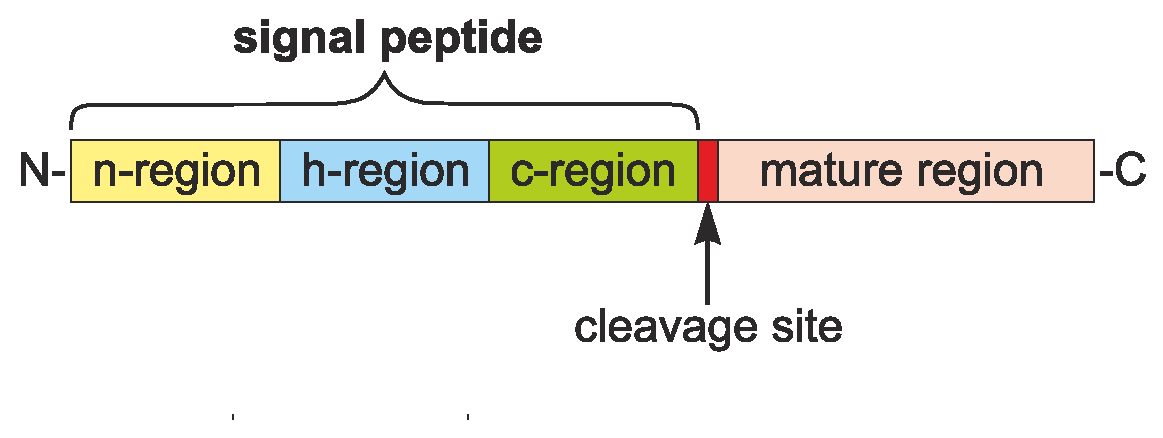
\includegraphics[width=0.55\textwidth]{figures/SP.eps}
\caption{The organization of typical signal peptide. The regions are not drawn in scale.}
\label{fig:sparch}
\end{figure}


Some data indicate that signal peptides may be universal. It was found, for example, that even bacterial signal peptides targeted correctly transgenic proteins to plant~\cite{2009moellera} or mammalian secretory systems~\cite{2014naganoestablishment}. On the other hand, signal peptides show great variation and the description presented above (Fig. \ref{fig:sparch}) refers to the most ???typical’ signal peptides. There are  exceptionally long signal peptides, which fulfill more sophisticated roles~\cite{2009hissarchitecture}. The fragment of signal peptide from preprolactin takes part in the regulation of prolactin secretion, whereas signal peptides of MHC class I inhibit activity of NK cells. Signal peptides of viral origin are involved in the immune evasion or viral life cycle~\cite{2000kappposttargeting}. The signal peptide from midkine contributing to the tumor progression contains epitopes recognized by CD4+ T cells~\cite{2013kerzerhothe}. The functional significance of these targeting signals makes that the prediction of signal peptide-containing proteins is also an important step in the drug development~\cite{2005zhangalteration, 2012netoadeimproving, 2010moellerwetmilling}.


\subsection*{Software predicting signal peptides}

Although many experimental methods determining the subcellular localization of proteins were devised, they are time consuming and laborious. Therefore, signal peptides became the subject of many computational programs to their prediction. Many software incorporates 'black-box’ models, such as: neural networks~\cite{2011petersensignalp}, support vector machines~\cite{2014zhangprediction}, Bayesian networks~\cite{2012zhengsignalbnf} or k-nearest neighbours~\cite{2007shensignall}. However, these models do not provide direct biological information about organization of signal peptides and are not able to predict properly atypical signal peptides. Although there are programs that do not share the innate flaws of 'black-box' models, they also demand an improvement. Some of them are based on position matrices or their variants~\cite{2014zhangprediction, 2004hillerpredisi}. Others (Phobius, Philius and SignalP 3.0) use hidden Markov models (HMMs)~\cite{2004klla, 2008reynoldstransmembrane, 2004bendtsenimproved}, which try to reflect structure of signal peptides regions in their limited probabilistic frameworks. The used HMMs, however, imply a geometric distribution for duration of regions length. We studied the distribution for regions from the first work utilizing HMMs in prediction of signal peptides~\cite{1998nielsenprediction} and found that the length distribution for every region was not geometric (Fig. \ref{fig:reglen}). Moreover, the commonly used rigid scheme of signal peptide's organization (Fig. \ref{fig:sparch}) does not describe extremely long or short peptides. Theoretically, HMMs that describe the atypical signal peptides could be developed to consider also the unusual structures but such probabilistic frameworks have not yet been implemented.

\begin{figure}[ht]\centering
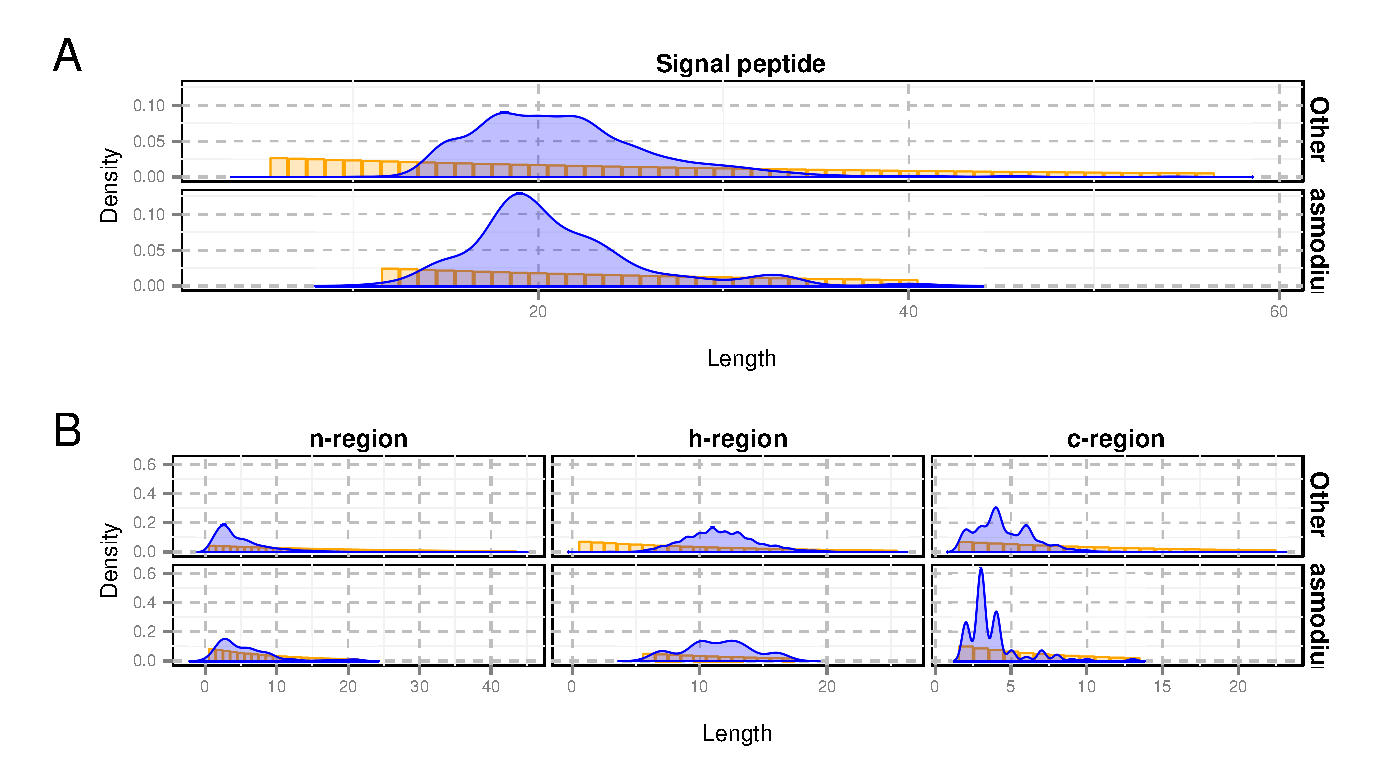
\includegraphics[width=0.95\textwidth]{figures/reglen.eps}
\caption{Distribution of lengths of signal peptides (A) and their regions (B) expressed in the number of amino acid residues. The data was extracted from 2~589 signal peptide sequences derived from UniProt database (see \textbf{Data selection} in \textbf{Methods}).}
\label{fig:reglen}
\end{figure}

All programs used in signal peptide recognition are trained on real protein sequences. Therefore, they succeed in the recognition of peptides similar to those in the learning set but fail in the case of artificial signal peptides. Such peptides are designed to increase effectiveness of protein secretion~\cite{2010futatsumorisugaisignal}. They are especially important in industrial applications to increase yield of proteins. Therefore, only explicit knowledge about the organization of signal peptides allows creating sequences that will be the most efficient in the export of proteins~\cite{2013ngengineering}. Signal peptides have also an important application in gene therapy. Mimicking the natural mechanism of protein export, artificial signal peptides with tumor epitopes increase the antitumor immune response~\cite{2003heenhanced}. Such epitopes must be properly inserted into a signal peptide without decreasing its secretion properties through disruption of the regional structure. Instead of time-consuming and expensive laboratory experiments, it would be very useful to survey \textit{in silico} many artificial peptides to select the ones that would fulfill the designed role.

Majority of the signal peptide predicting software uses the orthogonal encoding of amino acids, in which a vector of 20 digits represents every amino acid. This method of encoding, however, does not take into account relationships between amino acids and differences in their physicochemical properties. This is disadvantage of such signal peptide models because their regions are in fact characterized by specific features of amino acid residues and not by the simple occurrence of specific amino acids. In addition to this, such sparse encoding enforces larger data sets, which hinders their management and analysis~\cite{2002linamino}. Therefore, we elaborated a new approach based on hidden semi-Markov models using grouping of amino acids into physicochemical groups characteristic of signal peptides. The new methods proved better in comparison to the current software.

\section*{Methods}

\subsection*{Overview}

Since the functionality of signal peptides depends on the physicochemical properties of residues in a given region, we clustered amino acids into several groups based on their characteristics. The pre-processed sequences were further analyzed by the heuristic algorithm, which determines borders between three characteristic signal peptide regions~\cite{1998nielsenprediction}. We refined some region recognition criteria to attune the algorithm to less typical signal peptides. Next, two models were trained to recognize proteins with and without a signal peptide. The first one was a hidden semi-Markov model, in which each of three signal peptide regions was represented by a different hidden state. The additional fourth hidden state represented a mature protein. Each state was described by its frequencies of amino acid groups. The distribution of hidden states durations, i.e. the number of amino acids, was based on the empirical distribution of region lengths from the training set. Furthermore, the hidden semi-Markov model was enriched with n-grams representing signal peptide cleavage sites. The second model was a simple probabilistic approach in which no association between amino acids was assumed, and probability of amino acids groups occurrence was determined by their frequencies in mature proteins.

\subsection*{Data selection}

Eukaryotic protein sequences and their annotations were downloaded from UniProt database release 2015\_06. The preparations included the usual removal of sequences with more than one cleavage site, unknown cleavage site position, ambiguous symbols: X, J, Z, B or selenocysteine (U) from the final data set. The positive set contained 102 sequences with a signal peptide, containing its start and cleavage site information. The negative set comprised 358 sequences without any signal peptide annotation. All proteins belonged to the organisms from Plasmodiidae family.



\subsection*{Clustering of amino acids}

signalHsmm is not the first software which uses amino acid encoding in signal peptide prediction. BLOMAP~\cite{maetschke2005blomap} also employed the similar strategy but considered only substitution matrices. However, we applied different approach. We clustered amino acids using four properties relevant for the architecture of signal peptide: their hydrophobicity, frequency in $\alpha$-helices, polarity and size. The high hydrophobicity is a determinant of the h-region, whose $\alpha$-helix secondary structure is probably induced by the positively charged n-region. The high polarity as well as small size are important features of residues in the cleavage site~\cite{1994palzkillselection}.

\begin{table}[ht]
\small
\centering
\caption{Properties used in amino acid clusterization.} 
\begin{tabular}{ll}
  \toprule
Property name & Amino acid scale and its reference \\ 
  \midrule
Size & Size~\cite{dawson1972size} \\ 
   \rowcolor[gray]{0.85}Size & Molecular weight~\cite{fasman1976handbook}\\ 
  Size & Residue volume~\cite{1973goldsackcontribution} \\ 
   \rowcolor[gray]{0.85}Size & Bulkiness~\cite{1968zimmermanthe} \\ 
  Hydrophobicity & Normalized hydrophobicity scales for $\alpha$-proteins~\cite{1992cidhydrophobicity} \\ 
   \rowcolor[gray]{0.85}Hydrophobicity & Consensus normalized hydrophobicity scale~\cite{1984eisenbergthreedimensional} \\ 
  Hydrophobicity & Hydropathy index~\cite{1982kytea} \\ 
   \rowcolor[gray]{0.85}Hydrophobicity & Surrounding hydrophobicity in $\alpha$-helix~\cite{1980ponnuswamyhydrophobic} \\ 
  Polarity & Polarity~\cite{1974granthamamino} \\ 
   \rowcolor[gray]{0.85}Polarity & Mean polarity~\cite{1988radzickainfluences} \\ 
  Frequency in $\alpha$-helices & Signal sequence helical potential~\cite{1982argosstructural} \\ 
   \rowcolor[gray]{0.85}Frequency in $\alpha$-helices & Normalized frequency of N-terminal helix~\cite{chou1978prediction} \\ 
  Frequency in $\alpha$-helices & Relative frequency in $\alpha$-helix~\cite{1990prabhakaranthe} \\ 
   \bottomrule
\end{tabular}
\label{tab:aaprop}
\end{table}

We considered in total 13 amino acid scales from AAIndex database~\cite{2008kawashimaaaindex} (Tab.~\ref{tab:aaprop}). We selected one scale per property and carried out all possible 96 permutations of them. Based on that, we created 96 possible clusterings of amino acids using Euclidean distance and Ward's method. Next, we cut the clusterings to create four group of amino acids. In 31\% of cases, the groupings were identical. To compare the usefulness of encodings, we performed a 5-fold cross-validation training the new instance of signalHsmm on every encoding. We created balanced data sets by subsampling proteins without a signal peptide to equal the number of proteins with a signal peptide. The cross-validation was repeated 60 times to ensure that every protein without signal peptide was included in the learning set with the probability higher than 0.5. Very small variance of performance measures (for example see Tab.~\ref{tab:perfmeas})  confirmed the credibility of cross-validation.

\subsection*{Hidden semi-Markov model}
Hidden semi-Markov model (HSMM) is an extension of hidden Markov model (HMM). 
Let us first briefly describe the idea of the HMM. 
Suppose we have a sequence of observations, e.g. amino acids, and we are interested in understanding an underlying cause of their occurrence. 
HMM aims to answer that question assuming a specific and yet flexible structure of the problem.
HMM consists of two stochastic processes. The first is a discrete Markov chain $X_{t=1}^T$ on the set of so called hidden states $\{S_1, \dots S_n\}$.
They are "the cause" of the observations. At every step $t$, hidden state might change according to a transition matrix
$A= (a)_{i,j=1}^n$, where $a_{i,j} = \mathcal{P}(X_{t+1} = S_j | X_t = S_i)$. In our application, hidden states are signal peptide regions.
The second process $E_{t=1}^T$ is an observation process defined on the set of possible observations $\{O_1, \dots, O_m\}$. They are assumed to occur independently and conditionally on the hidden state that emits it. 
Their distribution are given by a matrix $B$, $b_{i,k} = \mathcal{P}(E_t = O_k | X_t = S_i)$.
In our case, the observations are (encoded) amino acids.
The main goal in signalHsmm is to find the most probable regions boundaries for a given peptide. This is achieved with Viterbi algorithm.
For a good reference on HMM see~\cite{1989rabinera}.

In the regular HMM, the hidden state duration, i.e. the number of observations emitted by the hidden state, has a geometric distribution. \cite{Durbin98biologicalsequence} showed how to extend it for different distributions without significant increase in computational 
complexity. Similar ideas were used for signal peptide recognition, for example by~\cite{2004klla}. 
However, it is still not flexible enough because the empirical regional length distributions (see Fig.~\ref{fig:reglen})
are difficult to capture in this way.

%rysunek pokazujący o co chodzi w HMM
\begin{figure}[h]
\centering
\tikzstyle{block} = [draw,shape=circle, top color=green!50!white!70, bottom color=green!50!white!70 ,minimum size=4em]
\tikzstyle{blockComp} = [draw,shape=circle, top color=red!50!white!70, bottom color=red!50!white!70 ,minimum size=2.5em]
% diameter of semicircle used to indicate that two lines are not connected
\def\radius{.7mm} 
\tikzstyle{branch}=[shape=rectangle, top color=white, bottom color=white ,minimum size=3pt,inner sep=0pt]
\tikzstyle{branch2}=[shape=rectangle, top color=white, bottom color=white ,minimum size=3pt,inner sep=0pt]
\def\n{11}
 \tikzstyle{line} = [draw=black, color=black!70!white!50, line width=1.5mm, -latex'] 
 \tikzstyle{line2} = [draw=black, color=red!30!white!70, line width=1.5mm, -latex']
\tikzstyle{frame}=[text=black,above, bottom color=white, top color=blue!50!black!70  ]
\tikzstyle{frameComp}=[text=black,below, bottom color=red!50!white!70, top color=red!50!white!70  ]
 \tikzstyle{line3} = [color=green!50!black!70, line width=1.5mm]
\def\names{{"$O_{1,1}$","...","$O_{1,d_1}$", "...","$O_{k, 1}$", "...", "$O_{k, d_k}$"}}%
\begin{tikzpicture}[>=latex']
%wąsate nawiasy
\draw [decorate, decoration={brace,amplitude=10pt},line3,xshift=0pt,yshift=0pt] (2.5,1) -> (10.5,1) node [branch,midway,yshift=0.8cm,color=black] 
	{\textbf{Hidden states}};
% \draw [->,decoration={brace,mirror,amplitude=10pt},line2,xshift=0pt,yshift=0pt] (11,-3) -- (3,-3) node [branch2,midway,yshift=-0.6cm,color=black] 
% 	{\textbf{Kierunek odczytu na nici Cricka ($3' \to 5'$)}}; 
   % Draw blocks, inputs and outputs
 
\node[block, text width=3em] at (1+2,0) (block1) {\footnotesize 1st hidden state};
\node[blockComp] at (-.5+2,-2)  (komp1) {\footnotesize \pgfmathparse{\names[0]}\pgfmathresult};
\node[blockComp] at (1+2,-2)  (komp2) {\footnotesize \pgfmathparse{\names[1]}\pgfmathresult};
\node[blockComp] at (2.5+2,-2)  (komp3) {\footnotesize \pgfmathparse{\names[2]}\pgfmathresult};
\draw[line,->]  (block1) --  (komp1);
\draw[line,->]  (block1) --  (komp2);
\draw[line,->]  (block1) --  (komp3);
\draw[line3,->] (block1.east) -- +(2,0) node [branch,midway,yshift=0.3cm,xshift=-0.2cm,color=black] {\footnotesize \textbf{transition}};

\node[block, bottom color=green!50!white!80,] at (4.5+2,0) (block2) {...};
\draw[line3,->] (block2.east) -- +(2,0) node [branch,midway,yshift=0.3cm,xshift=-0.2cm,color=black] {\footnotesize \textbf{transition}};
\node[blockComp] at (4.5+2,-2)  (komp4) {\footnotesize \pgfmathparse{\names[3]}\pgfmathresult};
\draw[line,->]  (block2) --  (komp4) ;

\node[block,text width=3em, bottom color=green!50!white!70] at (8+2,0) (block3) {\footnotesize $k^{th}$ hidden state};
\node[blockComp] at (6.5+2,-2)  (komp5) {\footnotesize \pgfmathparse{\names[4]}\pgfmathresult};
\node[blockComp] at (8+2,-2)  (komp6) {\footnotesize \pgfmathparse{\names[5]}\pgfmathresult};
\node[blockComp] at (9.5+2,-2)  (komp7) {\footnotesize \pgfmathparse{\names[6]}\pgfmathresult};
\draw[line,->]  (block3) --  (komp5);
\draw[line,->]  (block3) --  (komp6);
\draw[line,->]  (block3) --  (komp7);

% \draw[<->, color=red!30!black!50, line width=1.5mm] (komp1) |- +(5,-1.5) node[line2, yshift=-0.5cm] {\textbf{Observations}} -| (komp7); 

\draw [color=red!50!black!70, line width=1.5mm, decorate,decoration={brace,amplitude=10pt,mirror,raise=10pt},yshift=-10pt]
(1,-1.8) -- (5,-1.8) node [branch2, midway, yshift=-1cm,color=black] {\textbf{Duration of length $d_1$}};

\draw [color=red!50!black!70, line width=1.5mm, decorate,decoration={brace,amplitude=10pt,mirror,raise=10pt},yshift=-10pt]
(8,-1.8) -- (12,-1.8) node [branch2, midway, yshift=-1cm,color=black] {\textbf{Duration of length $d_k$}};

\draw [color=red!50!black!70, line width=1.5mm, decorate,decoration={brace,amplitude=15pt,mirror,raise=10pt},yshift=-10pt]
(1,-2.6) -- (12,-2.6) node [branch2, midway, yshift=-1.3cm,color=black] {\textbf{Observations, $\sum_{i=1}^k d_i = T$}};
\end{tikzpicture}
\caption{General scheme of hidden semi-Markov model.}
\label{fig:hsmm}
\end{figure}


The model we used is Hidden semi-Markov Model (HSMM)~\cite{Yu2010215}. It extends HMM by allowing any given hidden state duration distribution (Fig.~\ref{fig:hsmm}).
In addition to matrices $A$ and $B$, the model is given by probabilities of duration length in hidden states.
$$\mathcal{P}(\text{duration in state} = d | \text{state is } S_i), \;\; i = 1, \dots, n, \;\; d = 1, \dots, D$$
where $D$ is the maximum allowed duration.
As our datasets are of reasonable size and $D$ is small -- around 30, computational effort is not much 
higher than in the regular HMM. 

Our model has a very specific structure. The hidden states represent signal peptide regions.
Almost all entries in the transition matrix $A$ are zeros because regions are sequential.
Possible transitions are depicted as arrows in Fig.~\ref{fig:ngramext}.
Probabilities of observations for the hidden states and hidden states durations were estimated from training data.
The advantage of HSMM model is not only a better performance but also its straightforwardness.
Fig.~\ref{fig:ngramext} is easy to interpret for a researcher without any mathematical background.

%model structure

\begin{figure}[ht]\centering

\includegraphics[width=0.51\textwidth]{figures/HSMMs.eps}
\caption{The diagram of simple (A) and extended version of signalHsmm with the n-gram cleavage site model (B).}
\label{fig:ngramext}
\end{figure}

    
\subsection*{Extension of n-grams}

Hidden semi-Markov models may be flexibly enhanced by adding additional hidden states. To improve our model, we added few supplementary states representing specific motives that might occur in the proximity of cleavage site. The structure of cleavage sites, more conserved than other parts of signal peptide~\cite{2004hillerpredisi}, may be reflected by n-grams (k-mers), short vectors of $n$ characters derived from input sequences. Using the biogram software~\cite{biogramPackage}, we extracted n-grams from cleavage sites of signal peptides. The analyzed sequences were already encoded using amino acid classification providing the best sensitivity of the general model (Tab. \ref{tab:best}). Selected n-grams representing less common cleavage site motifs were included in the HSMM model as alternative paths at the end of c-region (Fig.~\ref{fig:ngramext}B).


\section*{Results and discussion}

\subsection*{Cross-validation}

\begin{figure}[ht]\centering
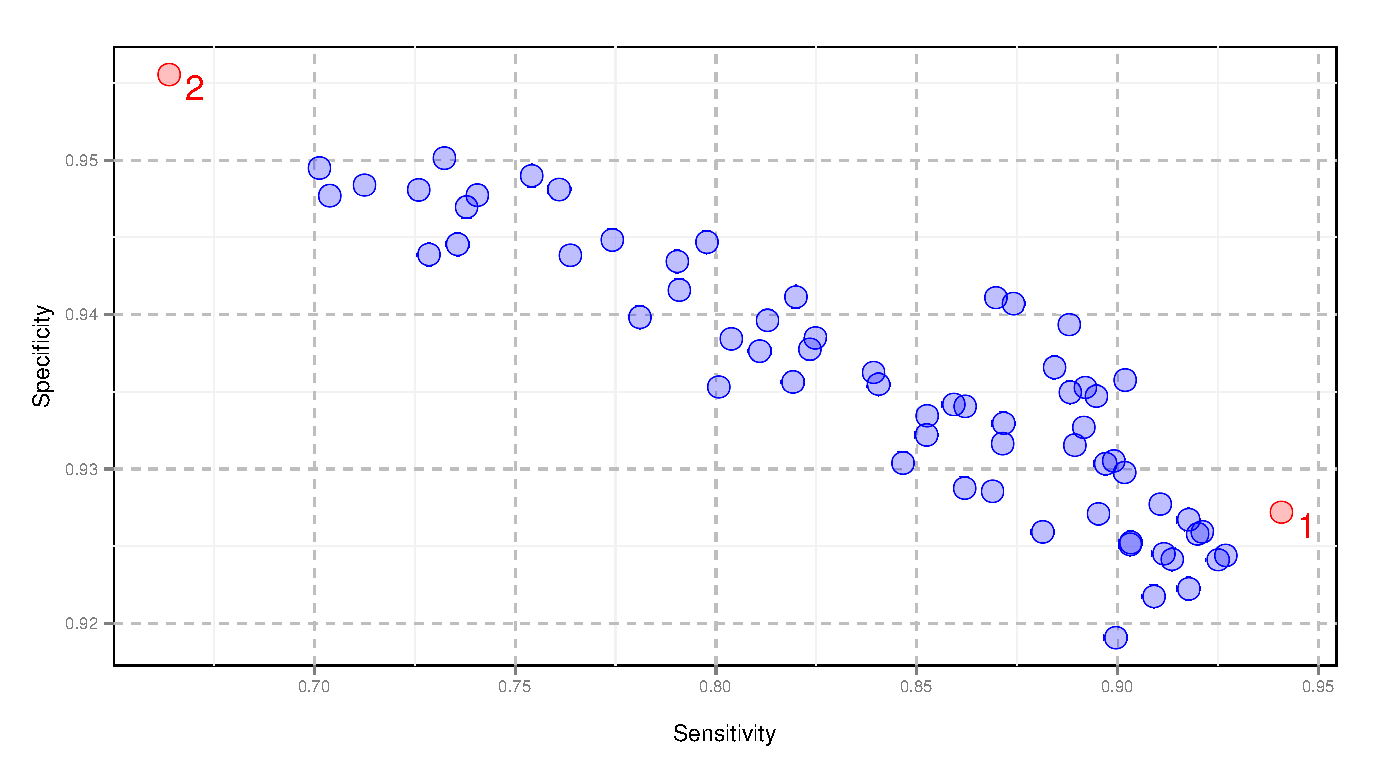
\includegraphics[width=0.95\textwidth, height=7cm]{figures/cvres.eps}
\caption{Sensitivity and specificity of amino acid encodings after cross-validation. 1 indicates the encoding providing the best sensitivity ($\textrm{AUC} = 0.9683$, $\textrm{MCC} = 0.8677$), whereas 2 means the encoding providing the best specificity ($\textrm{AUC} = 0.9338$, $\textrm{MCC} = 0.6474$).}
\label{fig:cvres}
\end{figure}

\begin{table}[ht]
\small
\begin{minipage}{.5\linewidth} 
\centering
\caption{The best sensitivity (final) encoding.} 
\begin{tabular}{l}
  \toprule
Groups \\ 
  \midrule
D, E, H, K, N, Q, R \\ 
   \rowcolor[gray]{0.85}G, P, S, T, Y \\ 
  F, I, L, M, V, W \\ 
   \rowcolor[gray]{0.85}A, C \\ 
   \bottomrule
\end{tabular}
\label{tab:best}
\end{minipage}
\begin{minipage}{.5\linewidth} 
\centering
\caption{The best specificity encoding.} 
\begin{tabular}{l}
  \toprule
Groups \\ 
  \midrule
A, E, K, Q, R \\ 
   \rowcolor[gray]{0.85}D, G, N, P, S, T \\ 
  C, H, I, L, M, V \\ 
   \rowcolor[gray]{0.85}F, W, Y \\ 
   \bottomrule
\end{tabular}
\label{tab:worst}
\end{minipage}
\end{table}


\begin{figure}[ht]\centering
%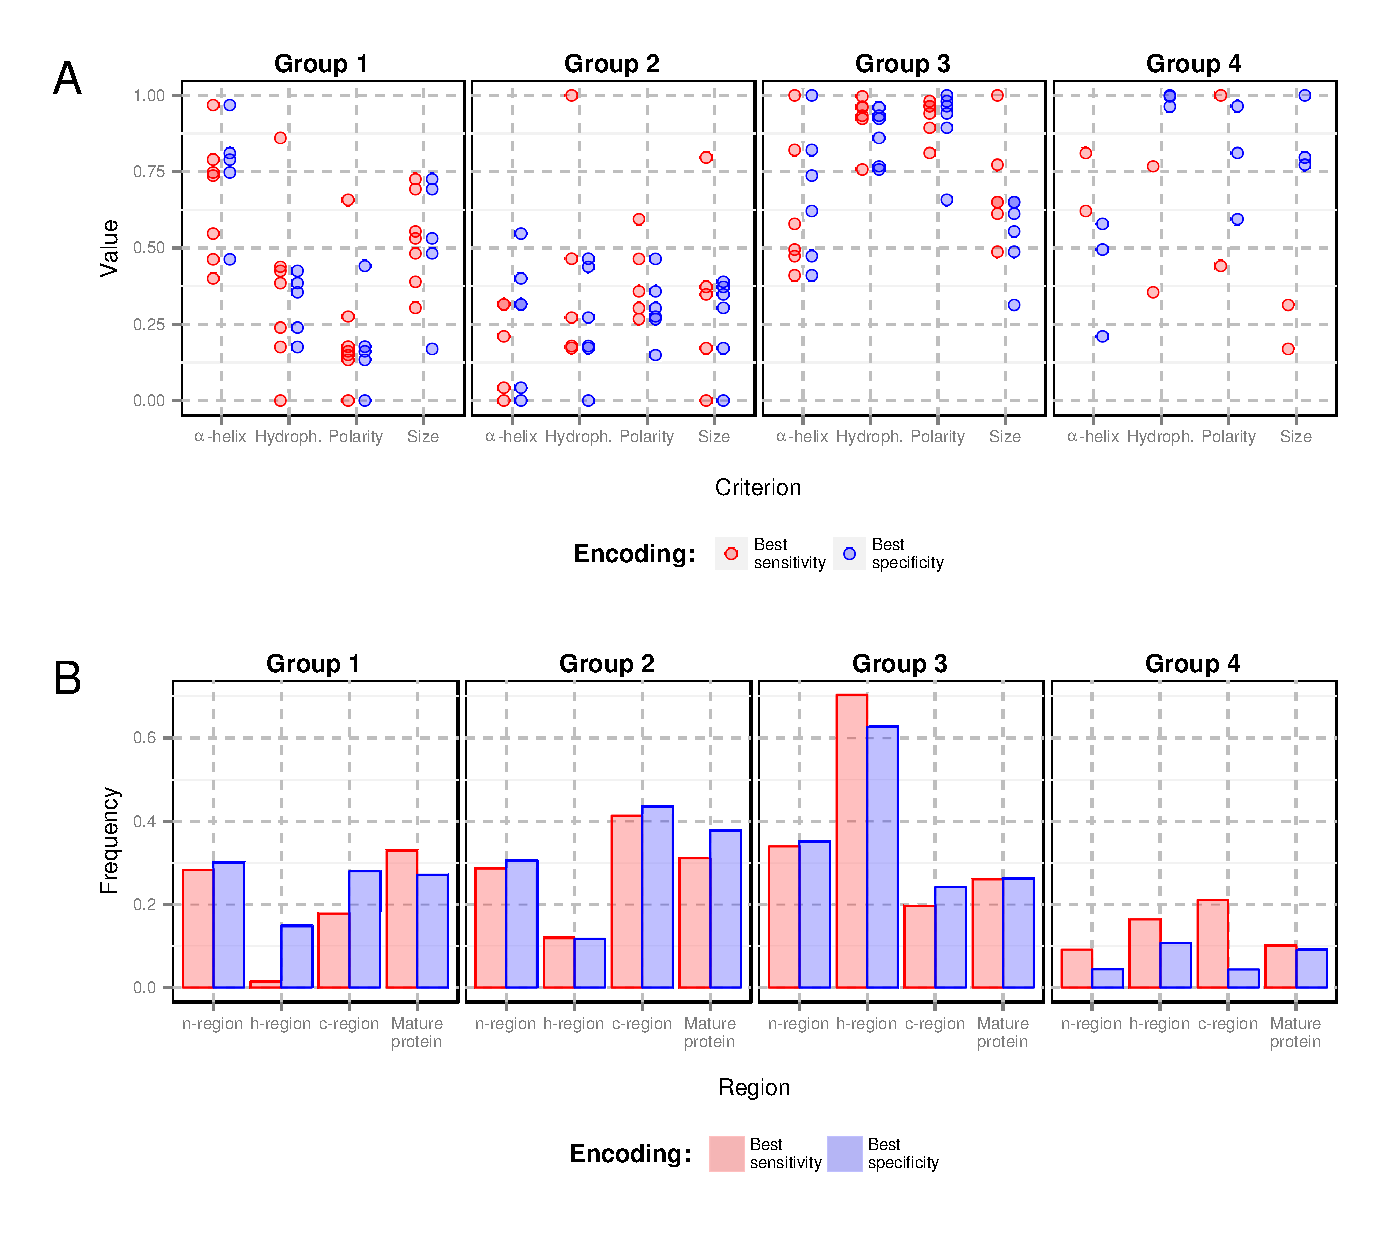
\includegraphics[width=0.95\textwidth]{figures/enccomp.eps}
\caption{Comparison of amino acid encodings with the best sensitivity and the best
specificity in different regions of signal peptide and mature proteins according to: A) the normalized value of properties for particular amino acids (points) and B) frequencies of amino acids in the given region.}
\label{fig:enccomp}
\end{figure}

We used four performance measures to evaluate results of cross-validation: specificity, sensitivity, Matthew's Correlation Coefficient ($\phi$ coefficient) and Area Under the Curve (AUC). All encodings provided very good AUC (0.93 -- 0.97) and specificity (0.92 -- 0.96). The classification of amino acids had the biggest impact on sensitivity, which ranges from 0.66 to 0.94. The final signalHsmm algorithm uses the encoding that yields the highest specificity and Matthew's Correlation coefficient as well as the second best AUC (Fig.~\ref{fig:cvres}).

\begin{table}[ht]
\small
\centering
\caption{Performance measures for the best encoding. 60 repetitions of cross-validation.} 
\begin{tabular}{lrr}
  \toprule
Measure & Mean & SD \\ 
  \midrule
AUC & 0.9683 & 0.0024 \\ 
   \rowcolor[gray]{0.85}MCC & 0.8677 & 0.0049 \\ 
  Sensitivity & 0.9406 & 0.0008 \\ 
   \rowcolor[gray]{0.85}Specificity & 0.9269 & 0.0050 \\ 
   \bottomrule
\end{tabular}
\label{tab:perfmeas}
\end{table}

\subsection*{Comparison of encodings}

We examined in detail encodings with the best sensitivity and the best specificity (Tab.~\ref{tab:best}, Tab.~\ref{tab:worst} and Fig.~\ref{fig:enccomp}). In both cases, the group 1 tends to contain average-sized polar amino acids. In the best sensitivity encoding, all charged amino acids, both acidic and basic (also weakly basic histidine)   belong to this group. These amino acids are nearly absent from h-region and provide very good distinction between regions of signal peptide (Fig.~\ref{fig:enccomp}). In the best specificity encoding, where polar and charged character of the group 1 is not so explicit, the difference in its distribution between the regions is also less visible.
The amino acids belonging to the group 2 have a quite low probability of occurrence in $\alpha$-helix and are very diverse. This group includes polar but uncharged serine and threonine as well as hydrophobic tyrosine, aliphatic glycine and proline. In the best specificity encoding, the polar character of this group is emphasized by the addition of asparagine and aspartic acid. Despite these differences, the distribution of group 2 seems to be comparable in two encodings. The both groupings have strongly non-polar and aliphatic group 3 containing isoleucine, leucine, methionine and valine. The hydrophobic property of this group in the best sensitivity encoding are even more pronounced by the presence of tryptophan and phenylalanine. On the contrary, more polar histidine belongs to the group 3 in the best specificity encoding. Because of the hydrophobic character, this group dominates in the h-region in the case of both amino acid classifications.
The fourth group is the most diverse in both encodings. In the case of the best specificity encoding, this group comprises aromatic amino acids: phenylalanine, tryptophan and tyrosine. In contrast, the group 4 in the best sensitivity encoding contains only alanine and cysteine, which both are rather small amino acids and tend to appear in $\alpha$-helices. This very unique composition seems to be typical of the c-region of signal peptide.

The encoding of amino acid plays crucial role in the recognition of signal peptide but does not affect identification of proteins without signal peptides (compare change in specificity and sensitivity on Fig.~\ref{fig:cvres}). The mature protein state in the HSMM model tends to have a more uniform distribution of residues than signal peptide region, which makes it more resistant to changes in amino acid groupings.

\subsection*{Benchmark tests}

To provide the honest comparison, we trained our model on 2311 signal peptide-containing sequences deposited in Uniprot until 2010 year (an iteration of signalHsmm called signalHsmm-2010). The data set should correspond to the set used to train SignalP 4.1. Interestingly, our algorithm performed very well even if it was trained on a very small sets including only 336 sequences collected till 1987 year, just after the first method predicting signal peptide was published~\cite{1986vonheijnea}. The signalHsmm-1987 was able to very accurately predict a signal peptide, even better than predictors trained on richer data sets. It indicates that signalHsmm is very stable and able to recover the structure of signal peptides from even very small data sets (Tab.~\ref{tab:bench2010}).

\begin{table}[ht]
\small
\centering
\caption{Comparison of Area Under the Curve, Sensitivity, Specificity and Matthews Correlation Coefficient for different classifiers.} 
\begin{tabular}{lrrrr}
  \toprule
Software name & AUC & Sensitivity & Specificity & MCC \\ 
  \midrule
signalP 4.1 (no tm) \cite{2011petersensignalp} & 0.9416 & \textbf{0.9720} & 0.9112 & 0.8848 \\ 
   \rowcolor[gray]{0.85}signalP 4.1 (tm) \cite{2011petersensignalp} & 0.9673 & 0.9579 & \textbf{0.9766} & \textbf{0.9347} \\ 
  PrediSi \cite{2004hillerpredisi} & 0.8949 & 0.9065 & 0.8832 & 0.7899 \\ 
   \rowcolor[gray]{0.85}Phobius \cite{2004klla} & 0.9509 & 0.9673 & 0.9346 & 0.9024 \\ 
  Philius \cite{2008reynoldstransmembrane} & 0.9369 & 0.9533 & 0.9206 & 0.8743 \\ 
   \rowcolor[gray]{0.85}signalHsmm-2010 & 0.9526 & 0.9533 & 0.8832 & 0.8385 \\ 
  signalHsmm-1989 & 0.9562 & 0.9626 & 0.8972 & 0.8617 \\ 
   \rowcolor[gray]{0.85}signalHsmm-2010 with k-mers & \textbf{0.9679} & 0.9673 & 0.9112 & 0.8799 \\ 
   \bottomrule
\end{tabular}
\label{tab:bench2010}
\end{table}

\begin{table}[ht]
\centering
\caption{Comparison of Area Under the Curve, H-measure and Matthews Correlation Coefficient for different classifiers considering only proteins belonging to Plasmodiidae.} 
\begin{tabular}{lrrrr}
  \toprule
Software name & AUC & Sensitivity & Specificity & MCC \\ 
  \midrule
signalP 4.1 (no tm) \cite{2011petersensignalp} & 0.8356 & 0.7745 & 0.8966 & 0.6420 \\ 
   \rowcolor[gray]{0.85}signalP 4.1 (tm) \cite{2011petersensignalp} & 0.7928 & 0.6471 & 0.9385 & 0.6185 \\ 
  PrediSi \cite{2004hillerpredisi} & 0.6597 & 0.3725 & 0.9469 & 0.4028 \\ 
   \rowcolor[gray]{0.85}Phobius \cite{2004klla} & 0.7963 & 0.6765 & 0.9162 & 0.5991 \\ 
  Philius \cite{2008reynoldstransmembrane} & 0.7753 & 0.6176 & 0.9330 & 0.5841 \\ 
   \rowcolor[gray]{0.85}signalHsmm-2010 & \textbf{0.9340} & \textbf{1.0000} & 0.8436 & \textbf{0.7380} \\ 
  signalHsmm-1989 & 0.9326 & 0.9510 & \textbf{0.8631} & 0.7266 \\ 
   \rowcolor[gray]{0.85}signalHsmm-2010 with k-mers & 0.9334 & 0.9902 & 0.7989 & 0.6767 \\ 
   \bottomrule
\end{tabular}
\label{tab:bench2010plas}
\end{table}

To check universality of our probabilistic model, we also validated it on signal peptides belonging to specific taxonomic groups. As an example, we chose the \textit{Plasmodiidae} family including malaria parasites because of their medical significance. The testing data set extracted from UniProt data base contained 102 sequences with a signal peptide and 358 sequences without it. Interestingly, signalHsmm showed much better performance than other algorithms (Tab.~\ref{tab:bench2010plas}). Since our algorithm considers more general decision rules, it is able to recognize also atypical signal peptides.


\subsection*{Conclusions}

The architecture of existing signal peptide predicting software is usually opaque, which unables to extract decision rules and determine parameters responsible for the predictions. Considering the biological context of the problem, we see a need for a transparent model of signal peptide. signalHsmm is the first step in this direction. 
It shows a good performance and provides clear interpretability and expendability of  the predictive algorithm. 
The model confirmed not only the high hydrophibicity of the h-region and polarity of the n-region but also found that alanine is one of the most typical amino acids in the c-region.
The performance of signalHsmm indicates that properties of signal peptides do not depend on their exact sequence but on the physicochemical features of the amino acids. 
The flexibility and efficient information recovery makes our model unique among similar software. signalHsmm is also adjustable to model properly very specific signal peptides belonging to taxonomic groups which are poorly represented in databases. Moreover, our method can effectively extract information from very small data sets, which in future may lead to new predictors specialized in recognition of atypical signaling sequences.

\subsection*{Availability and implementation}
The signalHsmm prediction web-server is available at: \url{http://smorfland.uni.wroc.pl/signalhsmm}. signalHsmm is implemented as an R package available at: \url{http://cran.r-project.org/web/packages/signalHsmm}. Stand-alone version offers prediction and tools to build, train and test novel signal peptide models.

\section*{Supporting Information}

% Include only the SI item label in the subsection heading. Use the \nameref{label} command to cite SI items in the text.
\subsection*{S1 Video}
\label{S1_Video}
{\bf Bold the first sentence.}  Maecenas convallis mauris sit amet sem ultrices gravida. Etiam eget sapien nibh. Sed ac ipsum eget enim egestas ullamcorper nec euismod ligula. Curabitur fringilla pulvinar lectus consectetur pellentesque.

\subsection*{S1 Text}
\label{S1_Text}
{\bf Lorem Ipsum.} Maecenas convallis mauris sit amet sem ultrices gravida. Etiam eget sapien nibh. Sed ac ipsum eget enim egestas ullamcorper nec euismod ligula. Curabitur fringilla pulvinar lectus consectetur pellentesque.

\subsection*{S1 Fig}
\label{S1_Fig}
{\bf Lorem Ipsum.} Maecenas convallis mauris sit amet sem ultrices gravida. Etiam eget sapien nibh. Sed ac ipsum eget enim egestas ullamcorper nec euismod ligula. Curabitur fringilla pulvinar lectus consectetur pellentesque.

\subsection*{S2 Fig}
\label{S2_Fig}
{\bf Lorem Ipsum.} Maecenas convallis mauris sit amet sem ultrices gravida. Etiam eget sapien nibh. Sed ac ipsum eget enim egestas ullamcorper nec euismod ligula. Curabitur fringilla pulvinar lectus consectetur pellentesque.

\subsection*{S1 Table}
\label{S1_Table}
{\bf Lorem Ipsum.} Maecenas convallis mauris sit amet sem ultrices gravida. Etiam eget sapien nibh. Sed ac ipsum eget enim egestas ullamcorper nec euismod ligula. Curabitur fringilla pulvinar lectus consectetur pellentesque.

\section*{Acknowledgments}
Cras egestas velit mauris, eu mollis turpis pellentesque sit amet. Interdum et malesuada fames ac ante ipsum primis in faucibus. Nam id pretium nisi. Sed ac quam id nisi malesuada congue. Sed interdum aliquet augue, at pellentesque quam rhoncus vitae.

\nolinenumbers

\section*{References}

\bibliography{lokalizom}


% Either type in your references using
% \begin{thebibliography}{}
% \bibitem{}
% Text
% \end{thebibliography}
%
% OR
%
% Compile your BiBTeX database using our plos2015.bst
% style file and paste the contents of your .bbl file
% here.
% 
% \begin{thebibliography}{10}
% \bibitem{bib1}
% Devaraju P, Gulati R, Antony PT, Mithun CB, Negi VS. Susceptibility to SLE in South Indian Tamils may be influenced by genetic selection pressure on TLR2 and TLR9 genes. Mol Immunol. 2014 Nov 22. pii: S0161-5890(14)00313-7. doi: 10.1016/j.molimm.2014.11.005
% 
% \bibitem{bib2}
% Huynen MMTE, Martens P, Hilderlink HBM. The health impacts of globalisation: a conceptual framework. Global Health. 2005;1: 14. Available: http://www.globalizationandhealth.com/content/1/1/14.
% 
% \end{thebibliography}



\end{document}

